\hypertarget{interacting-quantum-many-body-systems}{%
\section{Interacting Quantum Many Body Systems}\label{interacting-quantum-many-body-systems}}

When you take many objects and let them interact together, it is often simpler to describe the behaviour of the group in a different way to how one would describe the individual objects. Consider a flock of starlings like that of \cref{fig:Studland_Starlings}. Watching the flock you'll see that it has a distinct outline, that waves of density will sometimes propagate through the closely packed birds and that the flock seems to respond to predators as a distinct object. The natural description of this phenomena is in terms of the flock, not the individual birds.

The behaviours of the flock are an \emph{emergent phenomenon}. The starlings are only interacting with their immediate six or seven neighbours~\autocite{king2012murmurations,balleriniInteractionRulingAnimal2008}, what a physicist would call a \emph{local interaction}. There is much philosophical debate about how exactly to define emergence~\autocite{andersonMoreDifferent1972,kivelsonDefiningEmergencePhysics2016} but for our purposes it enough to say that emergence is the fact that the aggregate behaviour of many interacting objects may necessitate a description very different from that of the individual objects.

\hypertarget{fig:Studland_Starlings}{%
\begin{figure}
\centering
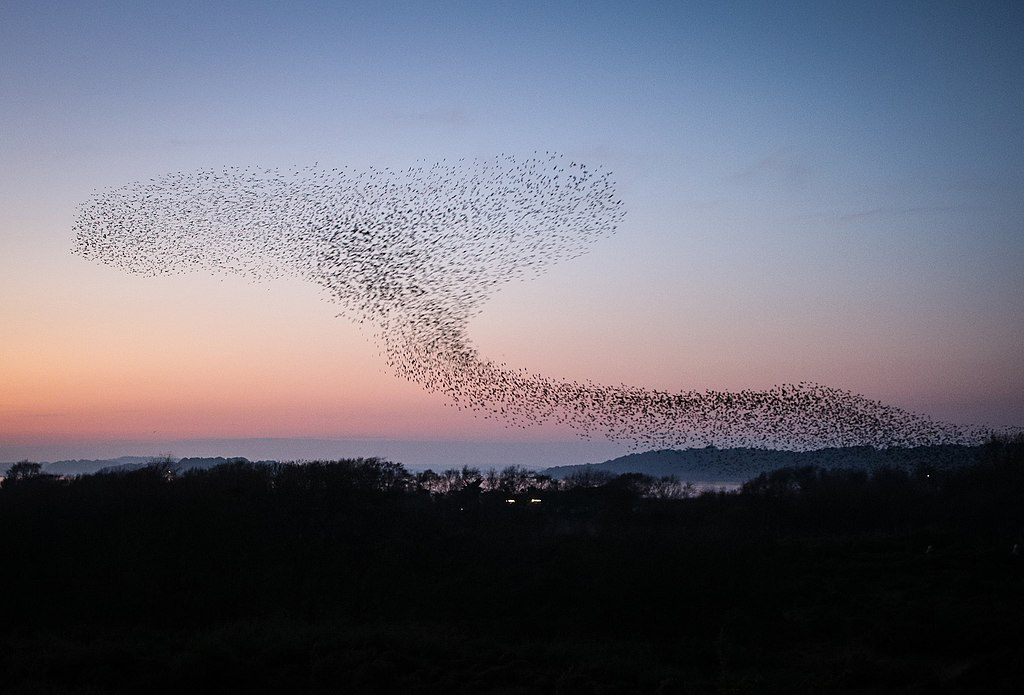
\includegraphics[width=1\textwidth,height=\textheight]{figure_code/intro_chapter/Studland_Starlings.jpeg}
\caption[{A murmuration of Starlings}]{A murmuration of starlings. Dorset, UK. Credit \href{https://twitter.com/arripay}{Tanya Hart}, ``Studland Starlings'', 2017, \href{https://creativecommons.org/licenses/by-sa/3.0/deed.en}{CC BY-SA 3.0}}
\label{fig:Studland_Starlings}
\end{figure}
}

To give an example closer to the topic at hand, our understanding of thermodynamics began with bulk properties like heat, energy, pressure and temperature~\autocite{saslowHistoryThermodynamicsMissing2020}. It was only later that we gained an understanding of how these properties emerge from microscopic interactions between very large numbers of particles~\autocite{flammHistoryOutlookStatistical1998}.

Condensed Matter is, at its heart, the study of what behaviours emerge from large numbers of interacting quantum objects at low energy. When these three properties are present together: a large number of objects, those objects being quantum and the presence interactions between the objects, we call it an interacting quantum many body system. From these three ingredients nature builds all manner of weird and wonderful materials.

Historically, we first made headway in the study of many-body systems, ignoring interactions and quantum properties. The ideal gas law and the Drude classical electron gas~\autocite{ashcroftSolidStatePhysics1976} are good examples. Including interactions too leads to the Ising model~\autocite{isingBeitragZurTheorie1925}, Landau theory~\autocite{landau2013fluid} and the classical theory of phase transitions~\autocite{jaegerEhrenfestClassificationPhase1998}. In contrast, condensed matter theory got its start in quantum many-body theory where the only electron-electron interaction considered is the Pauli exclusion principle. Bloch's theorem~\autocite{blochÜberQuantenmechanikElektronen1929}, the core result of band theory, predicted the properties of non-interacting electrons in crystal lattices, in particular that band insulators arise when the electrons bands are filled, leaving the fermi level in a bandgap~\autocite{ashcroftSolidStatePhysics1976}. In the same vein, advances were made in understanding the quantum origins of magnetism, including ferromagnetism and antiferromagnetism~\autocite{MagnetismCondensedMatter}.

The development of Landau-Fermi Liquid theory explained why band theory works so well even in cases where an analysis of the relevant energies suggests that it should not~\autocite{wenQuantumFieldTheory2007}. Landau Fermi Liquid theory demonstrates that in many cases where electron-electron interactions are significant, the system can still be described in terms of generalised non-interacting quasiparticles. This happens when the properties of the quasiparticles in the interacting system can be smoothly connected to the free fermions of the non-interacting system.

However there are systems where even Landau Fermi Liquid theory fails. An effective theoretical description of these systems must include electron-electron correlations and they are thus called Strongly Correlated Materials~\autocite{morosanStronglyCorrelatedMaterials2012}. The canonical examples are superconductivity~\autocite{MicroscopicTheorySuperconductivity}, the fractional quantum hall effect~\autocite{feldmanFractionalChargeFractional2021} and the Mott insulators~\autocite{mottBasisElectronTheory1949,fisherMottInsulatorsSpin1999}. We'll start by looking at the latter but shall see that there are many links between the three topics.

\hypertarget{mott-insulators}{%
\section{Mott Insulators}\label{mott-insulators}}

Mott Insulators are remarkable because their electrical insulator properties come not from having filled bands but from electron-electron interactions other than Pauli exclusion. Electrical conductivity, the bulk movement of electrons, requires both that there are electronic states very close in energy to the ground state and that those states are delocalised so that they can contribute to macroscopic transport. Band insulators are systems whose Fermi level falls within a gap in the density of states and thus fail the first criteria. Band insulators derive their character from the characteristics of the underlying lattice. A third kind of insulator, the Anderson Insulators, have only localised electronic states near the fermi level and therefore fail the second criteria. We will discuss Anderson insulators and the disorder that drives them, in a later section.

Both band and Anderson insulators occur without electron-electron interactions. Mott insulators, by contrast, require a many body picture to understand and thus elude band theory and single-particle methods.

\hypertarget{fig:venn_diagram}{%
\begin{figure}
\centering
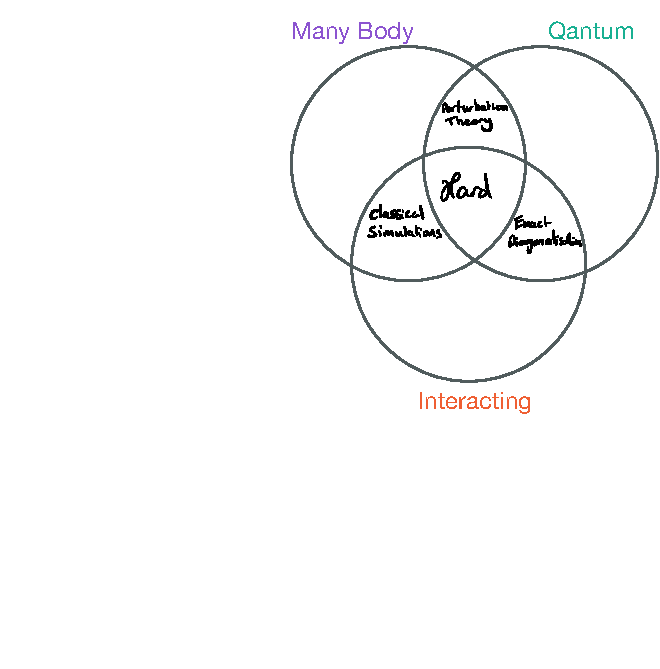
\includegraphics[width=1\textwidth,height=\textheight]{figure_code/intro_chapter/venn_diagram}
\caption[{Interacting Quantum Many Body Systems Venn Diagram}]{Three key adjectives. \emph{Many Body} refers to systems considered in the limit of large numbers of particles. \emph{Quantum}, objects whose behaviour requires quantum mechanics to describe accurately. \emph{Interacting}, the constituent particles of the system affect one another via forces, either directly or indirectly. When taken together, these three properties can give rise to what are called strongly correlated materials.}
\label{fig:venn_diagram}
\end{figure}
}

The theory of Mott insulators developed out of the observation that many transition metal oxides are erroneously predicted by band theory to be conductive~\autocite{boerSemiconductorsPartiallyCompletely1937} leading to the suggestion that electron-electron interactions were the cause of this effect~\autocite{mottDiscussionPaperBoer1937}. Interest grew with the discovery of high temperature superconductivity in the cuprates in 1986~\autocite{bednorzPossibleHighTcSuperconductivity1986} which is believed to arise as the result of a doped Mott insulator state~\autocite{leeDopingMottInsulator2006}.

The canonical toy model of the Mott insulator is the Hubbard model~\autocite{gutzwillerEffectCorrelationFerromagnetism1963,kanamoriElectronCorrelationFerromagnetism1963,hubbardj.ElectronCorrelationsNarrow1963} of spin-\(1/2\) fermions hopping on the lattice with hopping parameter \(t\) and electron-electron repulsion \(U\)

\[ H_{\mathrm{H}} = -t \sum_{\langle i,j \rangle \alpha} c^\dagger_{i\alpha} c_{j\alpha} + U \sum_i n_{i\uparrow} n_{i\downarrow} - \mu \sum_{i,\alpha} n_{i\alpha},\]

where \(c^\dagger_{i\alpha}\) creates a spin \(\alpha\) electron at site \(i\) and the number operator \(n_{i\alpha}\) measures the number of electrons with spin \(\alpha\) at site \(i\). The sum runs over lattice neighbours \(\langle i,j \rangle\) including both \(\langle i,j \rangle\) and \(\langle j,i \rangle\) so that the model is Hermition.

In the non-interacting limit \(U << t\), the model reduces to free fermions and the many-body ground state is a separable product of Bloch waves filled up to the Fermi level. In the interacting limit \(U >> t\) on the other hand, the ground state is a direct product of the local Hilbert spaces \(|0\rangle, |\uparrow\rangle, |\downarrow\rangle, |\uparrow\downarrow\rangle\). At half filling, one electron per site, each site becomes a \emph{local moment} in the reduced Hilbert space \(|\uparrow\rangle, |\downarrow\rangle\) and thus acts like a spin-\(1/2\)~\autocite{hubbardElectronCorrelationsNarrow1964}.

The Mott insulating phase occurs at half filling \(\mu = \tfrac{U}{2}\). Here the model can be rewritten in a symmetric form \[ H_{\mathrm{H}} = -t \sum_{\langle i,j \rangle \alpha} c^\dagger_{i\alpha} c_{j\alpha} + U \sum_i (n_{i\uparrow} - \tfrac{1}{2})(n_{i\downarrow} - \tfrac{1}{2}).\]

The basic reason that the half filled state is insulating seems trivial. Any excitation must include states of double occupancy that cost energy \(U\), hence the system has a finite bandgap and is an interaction driven Mott insulator. Depending on the lattice, the local moments may then order antiferromagnetically. Originally it was proposed that this antiferromagnetic (AFM) order was actually the reason for the insulating behaviour. This would make sense since AFM order doubles the unit cell and can turn a system into a band insulator with an even number of electrons per unit cell~\autocite{mottMetalInsulatorTransitions1990}. However, Mott insulators have been found~\autocite{law1TTaS2QuantumSpin2017,ribakGaplessExcitationsGround2017} without magnetic order. Instead the local moments may form a highly entangled state known as a quantum spin liquid, which will be discussed shortly.

Various theoretical treatments of the Hubbard model have been made, including those based on Fermi liquid theory, mean field treatments, the local density approximation (LDA)~\autocite{slaterMagneticEffectsHartreeFock1951}, dynamical mean-field theory~\autocite{greinerQuantumPhaseTransition2002}, density matrix renormalisation group methods~\autocite{hallbergNewTrendsDensity2006,schollwöckDensitymatrixRenormalizationGroup2005,whiteDensityMatrixFormulation1992} and Markov chain Monte Carlo~\autocite{blankenbeclerMonteCarloCalculations1981,hirschDiscreteHubbardStratonovichTransformation1983,whiteNumericalStudyTwodimensional1989}. None of these approaches are perfect. Strong correlations are poorly described by the Fermi liquid theory and the LDA approaches while mean field approximations do poorly in low dimensional systems. This theoretical difficulty has made the Hubbard model a target for cold atom simulations~\autocite{mazurenkoColdatomFermiHubbard2017}.

From here the discussion will branch in two directions. First, we will discuss a limit of the Hubbard model called the Falikov-Kimball Model. Second, we will look at quantum spin liquids and the Kitaev honeycomb model.

\textbf{The Falikov-Kimball Model}

\hypertarget{fig:fk_schematic}{%
\begin{figure}
\centering
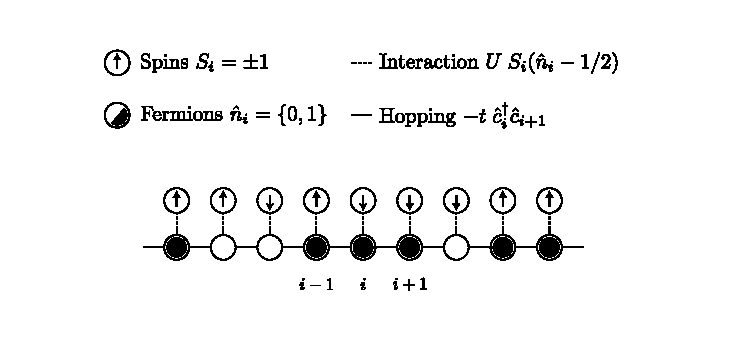
\includegraphics[width=1\textwidth,height=\textheight]{figure_code/intro_chapter/fk_schematic}
\caption[{Falicov-Kimball Model Diagram}]{The Falicov-Kimball Model can be viewed as a model of classical spins \(S_i\) coupled to spinless fermions \(\hat{c}_i\) where the fermions are mobile with hopping \(t\) and the fermions are coupled to the spins by an Ising type interaction with strength \(U\).}
\label{fig:fk_schematic}
\end{figure}
}

Originally introduced to describe the metal-insulator transition in f-electron system~\autocite{hubbardj.ElectronCorrelationsNarrow1963,falicovSimpleModelSemiconductorMetal1969}, the Falikov-Kimball (FK) model is the limit of the Hubbard model as the mass of one of the spins states of the electron is taken to infinity. This gives a model with two fermion species, one itinerant and one entirely immobile. The number operators for the immobile fermions are therefore conserved quantities and can be be treated like classical degrees of freedom. For our purposes it will be useful to replace the immobile fermions with a classical Ising background field \(S_i = \pm1\).

\[\begin{aligned}
H_{\mathrm{FK}} = & -\;t \sum_{\langle i,j \rangle} c^\dagger_{i}c_{j} + \;U \sum_{i} S_i\;(c^\dagger_{i}c_{i} - \tfrac{1}{2}). \\ 
\end{aligned}\]

Given that the physics of states near the metal-insulator (MI) transition is still poorly understood~\autocite{belitzAndersonMottTransition1994,baskoMetalInsulatorTransition2006} the FK model provides a rich test bed to explore interaction driven MI transition physics. Despite its simplicity, the model has a rich phase diagram in \(D \geq 2\) dimensions. It shows an Mott insulator transition even at high temperature, similar to the corresponding Hubbard Model~\autocite{brandtThermodynamicsCorrelationFunctions1989}. In 1D, the ground state phenomenology as a function of filling can be rich~\autocite{gruberGroundStatesSpinless1990} but the system is disordered for all \(T > 0\)~\autocite{kennedyItinerantElectronModel1986}. The model has also been a test-bed for many-body methods, interest took off when an exact dynamical mean-field theory solution in the infinite dimensional case was found~\autocite{antipovCriticalExponentsStrongly2014,ribicNonlocalCorrelationsSpectral2016,freericksExactDynamicalMeanfield2003,herrmannNonequilibriumDynamicalCluster2016}.

In~\protect\hyperlink{chap:3-the-long-range-falicov-kimball-model}{chapter 3} I will introduce a generalized Falikov-Kimball model in one dimension I call the Long-Range Falikov-Kimball model. With the addition of long-range interactions in the background field, the model shows a similarly rich phase diagram as its higher dimensional cousins. Our goal is to understand the Mott transition in more detail, the the phase transition into a charge density wave (CDW) state and how the localisation properties of the fermionic sector behave in one dimension. We were particularly interested to see if correlations in the disorder potential are enough to bring about localisation effects such mobility edges that are normally only seen in higher dimensions. I use an exact Markov chain Monte Carlo method to map the phase diagram and compute the energy-resolved localization properties of the fermions. We observe what seems like a hint of coexisting localised and delocalised states. However after careful comparison to an Anderson model of uncorrelated binary disorder about a background charge density wave field, we confirm that the fermionic sector does fully localize at larger system sizes as expected for one dimensional systems.

\hypertarget{quantum-spin-liquids}{%
\section{Quantum Spin Liquids}\label{quantum-spin-liquids}}

To turn to the other key topic of this thesis, we have already discussed the AFM ordering of local moments in the Mott insulating state. Landau-Ginzburg-Wilson theory characterises phases of matter as inextricably linked to the emergence of long range order via a spontaneously broken symmetry. So within this paradigm we would not expect any interesting phases of matter not associated with AFM or other long-range order. However, Anderson first proposed in 1973~\autocite{andersonResonatingValenceBonds1973} that if long range order is suppressed by some mechanism, it might lead to a liquid-like state even at zero temperature, the Quantum Spin Liquid (QSL).

This QSL state would exist at zero or very low temperatures, so we would expect quantum effects to be very strong, which will turn out to have far reaching consequences. It was the discovery of a different phase, however that really kickstarted interest in the topic. The fractional quantum Hall (FQH) state, discovered in the 1980s is an explicit example of an interacting electron system that falls outside of the Landau-Ginzburg-Wilson paradigm. It shares many phenomenological properties with the QSL state. They both exhibit fractionalised excitations, braiding statistics and non-trivial topological properties~\autocite{broholmQuantumSpinLiquids2020}. The many-body ground state of such systems acts as a complex and highly entangled vacuum. This vacuum can support quasiparticle excitations with properties unbound from that of the Dirac fermions of the standard model.

How do we actually make a QSL? Frustration is one mechanism that we can use to suppress magnetic order in spin models~\autocite{TrebstPhysRep2022}. Frustration can be geometric, triangular lattices for instance cannot support AFM order. It can also come about as a result of spin-orbit coupling or other physics. There are also other routes to QSLs besides frustrated spin systems that we will not discuss here~\autocite{balentsNodalLiquidTheory1998,balentsDualOrderParameter1999,linExactSymmetryWeaklyinteracting1998}.

\hypertarget{fig:kitaev-material-phase-diagram}{%
\begin{figure}
\centering
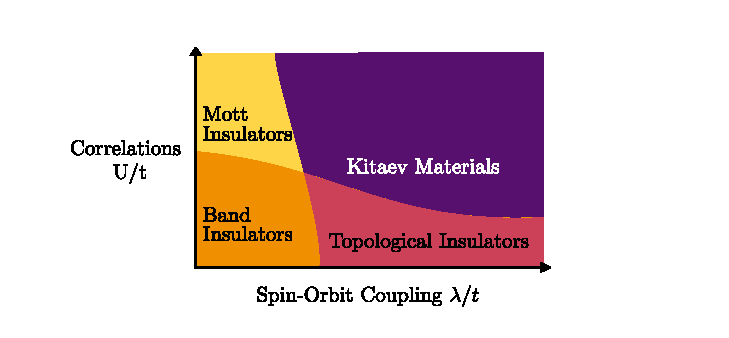
\includegraphics[width=1\textwidth,height=\textheight]{figure_code/intro_chapter/kitaev_material_phase_diagram}
\caption[{Phase Diagram}]{How Kitaev materials fit into the picture of strongly correlated systems. Interactions are required to open a Mott gap and localise the electrons into local moments, while spin-orbit correlations are required to produce the strongly anisotropic spin-spin couplings of the Kitaev Model. Reproduced from~\autocite{TrebstPhysRep2022}.}
\label{fig:kitaev-material-phase-diagram}
\end{figure}
}

Spin-orbit coupling is a relativistic effect that, very roughly, corresponds to the fact that in the frame of reference of a moving electron, the electric field of nearby nuclei looks like a magnetic field to which the electron spin couples. This effectively couples the spatial and spin parts of the electron wavefunction, meaning that the lattice structure can influence the form of the spin-spin interactions leading to spatial anisotropy in the effective interactions. This spatial anisotropy can frustrate the Mott insulators~\autocite{jackeliMottInsulatorsStrong2009,khaliullinOrbitalOrderFluctuations2005} leading to more exotic ground states than the AFM order we have seen so far. As we saw with the Hubbard model, interaction effects are only strong or weak in comparison to the bandwidth or hopping integral \(t\). Hence, we will see strong frustration in materials with strong spin-orbit coupling \(\lambda\) relative to their bandwidth \(t\).

In certain transition metal based compounds, such as those based on Iridium and Ruthenium, the lattice structure, strong spin-orbit coupling and narrow bandwidths lead to effective spin-\(\tfrac{1}{2}\) Mott insulating states with strongly anisotropic spin-spin couplings. These transition metal compounds, known as Kitaev Materials, draw their name from the celebrated Kitaev Honeycomb Model which is expected to model their low temperature behaviour~\autocite{Jackeli2009,HerrmannsAnRev2018,Winter2017,TrebstPhysRep2022,Takagi2019}.

At this point we can sketch out a phase diagram like that of \cref{fig:kitaev-material-phase-diagram}. When both electron-electron interactions \(U\) and spin-orbit couplings \(\lambda\) are small relative to the bandwidth \(t\) we recover standard band theory of band insulators and metals. In the upper left we have the simple Mott insulating state as described by the Hubbard model. In the lower right, strong spin-orbit coupling gives rise to Topological insulators (TIs) characterised by symmetry protected edge modes and non-zero Chern number. Kitaev materials occur in the region where strong electron-electron interaction and spin-orbit coupling interact. See~\autocite{witczak-krempaCorrelatedQuantumPhenomena2014} for a much more expansive version of this diagram.

The Kitaev Honeycomb model~\autocite{kitaevAnyonsExactlySolved2006} was the first exactly solvable spin model with a QSL ground state. It is defined on the two dimensional honeycomb lattice and provides an exactly solvable model that can be reduced to a free fermion problem via a mapping to Majorana fermions. This yields an extensive number of static \(\mathbb Z_2\) fluxes tied to an emergent gauge field. The model is remarkable not only for its QSL ground state but also for its fractionalised excitations with non-trivial braiding statistics. It has a rich phase diagram hosting gapless, Abelian and non-Abelian phases~\autocite{knolleDynamicsFractionalizationQuantum2015} and a finite temperature phase transition to a thermal metal state~\autocite{selfThermallyInducedMetallic2019}. It been proposed that its non-Abelian excitations could be used to support robust topological quantum computing~\autocite{kitaev_fault-tolerant_2003,freedmanTopologicalQuantumComputation2003,nayakNonAbelianAnyonsTopological2008}.

The Kitaev model and FK model have quite a bit of conceptual overlap. They are both effectively models of spinless fermions coupled to a classical Ising background field. This is what makes them exactly solvable. At finite temperatures, fluctuations in their background fields provides an effective disorder potential for the fermionic sector, so both models can be studied at finite temperature with Markov chain Monte Carlo methods~\autocite{antipovInteractionTunedAndersonMott2016,selfThermallyInducedMetallic2019}.

As Kitaev points out in his original paper, the model remains solvable on any tri-coordinated \(z=3\) graph which can be 3-edge-coloured. Indeed many generalisations of the model exist~\autocite{Baskaran2007,Baskaran2008,Nussinov2009,OBrienPRB2016,hermanns2015weyl}. Notably, the Yao-Kivelson model~\autocite{yaoExactChiralSpin2007} introduces triangular plaquettes to the honeycomb lattice leading to spontaneous chiral symmetry breaking. These extensions all retain translation symmetry, likely because edge-colouring, finding the ground state and understanding the QSL properties are much harder without it~\autocite{eschmann2019thermodynamics,Peri2020}. Undeterred, this gap lead us to wonder what might happen if we remove translation symmetry from the Kitaev Model. This might would be a model of a tri-coordinated, highly bond anisotropic but otherwise amorphous material.

Amorphous materials do not have long-range lattice regularities but covalent compounds can induce short-range regularities in the lattice structure such as fixed coordination number \(z\). The best examples being amorphous Silicon and Germanium with \(z=4\) which are used to make thin-film solar cells~\autocite{Weaire1971,betteridge1973possible}. Recently it has been shown that topological insulating (TI) phases can exist in amorphous systems. Amorphous TIs are characterized by similar protected edge states to their translation invariant cousins and generalised topological bulk invariants~\autocite{mitchellAmorphousTopologicalInsulators2018,agarwala2019topological,marsalTopologicalWeaireThorpeModels2020,costa2019toward,agarwala2020higher,spring2021amorphous,corbae2019evidence}. However, research on amorphous electronic systems has been mostly focused on non-interacting systems with a few exceptions, for example, to account for the observation of superconductivity~\autocite{buckel1954einfluss,mcmillan1981electron,meisel1981eliashberg,bergmann1976amorphous,mannaNoncrystallineTopologicalSuperconductors2022} in amorphous materials or very recently to understand the effect of strong electron repulsion in TIs~\autocite{kim2022fractionalization}.

Amorphous \emph{magnetic} systems have been investigated since the 1960s, mostly through the adaptation of theoretical tools developed for disordered systems~\autocite{aharony1975critical,Petrakovski1981,kaneyoshi1992introduction,Kaneyoshi2018} and with numerical methods~\autocite{fahnle1984monte,plascak2000ising}. Research on classical Heisenberg and Ising models has been shown to account for observed behaviour of ferromagnetism, disordered antiferromagnetism and widely observed spin glass behaviour~\autocite{coey1978amorphous}. However, the role of spin-anisotropic interactions and quantum effects in amorphous magnets has not been addressed.

In~\protect\hyperlink{chap:4-the-amorphous-kitaev-model}{chapter 4} I will address the question of whether frustrated magnetic interactions on amorphous lattices can give rise to genuine quantum phases, i.e.~to long-range entangled quantum spin liquids (QSL)~\autocite{Anderson1973,Knolle2019,Savary2016,Lacroix2011}. We will find that the answer is yes. I will introduce the Amorphous Kitaev (AK) model, a generalisation of the Kitaev honeycomb model to random lattices with fixed coordination number three. I will show that this model is a soluble, amorphous, chiral spin liquid. As with the Yao-Kivelson model~\autocite{yaoExactChiralSpin2007}, the AK model retains its exact solubility but the presence of plaquettes with an odd number of sides leads to a spontaneous breaking of time reversal symmetry. I will confirm prior observations that the form of the ground state is relatively simple~\autocite{OBrienPRB2016,eschmannThermodynamicClassificationThreedimensional2020} and unearth a rich phase diagram displaying Abelian as well as a non-Abelian chiral spin liquid phases. Furthermore, I show that the system undergoes a finite-temperature phase transition to a conducting thermal metal state and discuss possible experimental realisations.

The next chapter,~\protect\hyperlink{chap:2-background}{Chapter 2}, will introduce some necessary background to the Falikov-Kimball Model, the Kitaev Honeycomb Model, and disorder and localisation.
